\chapter{Reproducibility}
\label{app:repro}

Every run's checkpoint file records the configuration of
\Cref{tab:config} together with the input source path, the interval
$\tau$, and per-engine running totals, so that a resumed run can be
checked against the run it continues. A per-file input hash and a code
commit hash embedded in the run's own output --- which would let a
result be tied unambiguously to the exact code and data that produced
it, beyond what the configuration and file list already establish ---
are not currently written by the checkpoint format; this is listed here
as a gap worth closing, not implied to already exist. Given identical
input and configuration, an uninterrupted run reproduces identical
output in all columns except the two that measure computing time
(\Cref{sec:testdeterminism}); the month result is not such a run
(\Cref{sec:testresets}). The analysis pipeline reads only the
logged CSV output and is shared by both engines, so no metric is
computed by engine-specific code.

\section{Getting the Code}
\label{sec:repro_code}

\begin{sloppypar}
The full source, in Rust, is public \citep{moral2026marketsim}. It lives at
\url{https://github.com/alejandromoralwork/tfg}, branch \texttt{main}, commit
\ph[to be inserted before submission].
\end{sloppypar}
It is one crate, \texttt{market\_sim}, with no engine-specific dependency beyond
the standard Rust toolchain (edition 2021) --- both matching engines
(\texttt{src/engines/cda.rs}, \texttt{src/engines/fba.rs}), the binary decoder,
the metrics recorder and the command-line interface used below are plain
\texttt{.rs} files in that one repository, not a package pulled from elsewhere.
Cloning and building it is the same on any platform:

\begin{lstlisting}[language=,caption={Getting and building the simulator.}]
git clone https://github.com/alejandromoralwork/tfg.git
cd tfg/src
cargo build --release
# binary at target/release/market_sim (market_sim.exe on Windows)
\end{lstlisting}

With no arguments the binary drops into an interactive prompt; given arguments it
runs one command and exits, the form every automated run in this thesis used
(\texttt{main.rs}, the whole entry point):

\begin{lstlisting}[caption={The crate's entry point, in full.}]
fn main() {
    let args: Vec<String> = std::env::args().skip(1).collect();
    if args.is_empty() {
        inputs::cli::run();                          // interactive prompt
    } else {
        std::process::exit(inputs::cli::run_once(&args));   // one command, then exit
    }
}
\end{lstlisting}

\section{Running It Without Downloading Any Data}
\label{sec:repro_quick}

The repository carries a small, git-tracked sample (one hour of real SOL order
statuses, a few hundred thousand records) so the whole pipeline can be exercised
in well under a minute, with nothing downloaded first:

\begin{lstlisting}[language=,caption={A first run, on the bundled sample data.}]
market_sim simulate data/sample/order_statuses/20251201 1
# writes output/20251201/{fba,cda}_timeseries.csv, summary.txt, checkpoint.txt
market_sim test engine all
# 0 exit status only if all 37 hand-built checklist cases pass
\end{lstlisting}

\Cref{fig:cliscreenshot} shows the same binary's interactive prompt: switching
engine, adding orders by hand, reading back the book, and clearing an FBA batch,
exactly the commands and output described in \Cref{app:algorithm,tab:config}.
This is a real captured session; the terminal colours shown are reapplied from
the exact \texttt{.cyan()}/\texttt{.green()}/\dots calls in \texttt{src/inputs/cli.rs}
because the ANSI codes themselves are dropped when the output is piped into a file
rather than shown on a real terminal.

\begin{figure}[htbp]
\centering
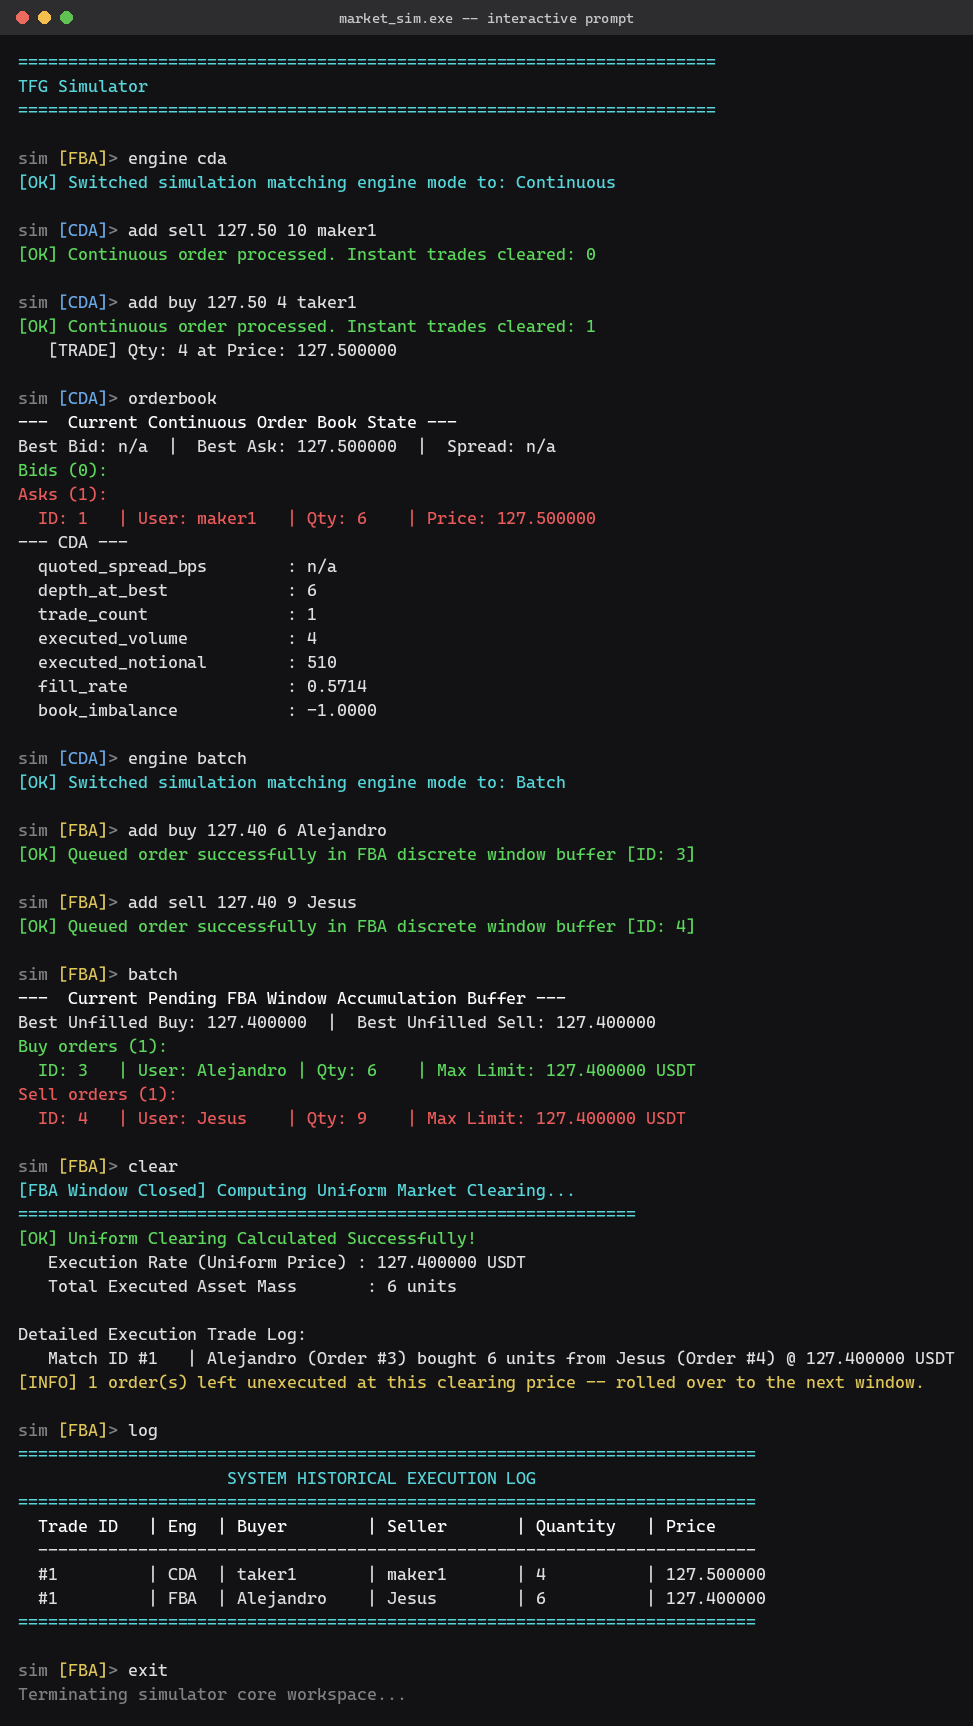
\includegraphics[width=0.92\textwidth]{figures/fig_cli_screenshot.png}
\caption[The simulator's interactive prompt]{A real session at the interactive
prompt: switching engine, adding orders, reading the book and the FBA buffer,
clearing a batch, and reading the combined trade log.}
\label{fig:cliscreenshot}
\end{figure}

\section{Running the Full Month}
\label{sec:repro_full}

Reproducing the actual results in \Cref{ch:results} needs the real December~2025
SOL archive (about 6\,GB compressed), fetched from the Zenodo record cited as
\citet{albers2026openbook}, at \url{https://zenodo.org/records/18184441}:

\begin{lstlisting}[language=,caption={Fetching the real dataset and replaying the whole month.}]
market_sim download sol            # fetches + extracts into data/order_statuses/sol
market_sim simulate sol 1          # the exact run behind this thesis; ~45h on one machine
\end{lstlisting}

A single machine is slow only because the replay is single-threaded by design
(\Cref{sec:environment}); the run can be stopped and resumed at any point, since
it checkpoints after every hourly file (\Cref{tab:config} above). For a faster
turnaround, \texttt{src/docs/DEPLOY.md} in the same repository is a complete,
copy-paste walkthrough for running the identical container on Google Cloud
Batch, including the exact job specification (\texttt{deploy/batch-sol.json})
this thesis's own cloud run used. It is written for a reader who has never used
Google Cloud before and takes them from installing \texttt{gcloud} to a finished
run in their own project, typically a few dollars of compute for the full month.

This thesis does not, and deliberately does not, publish a shared key or a
running virtual machine that lets a reader execute the simulation on the
author's own cloud account: a thesis PDF is effectively public forever, and a
live credential embedded in it cannot be safely revoked once distributed, while
leaving compute running for anonymous use is an open invitation to abuse and an
open-ended cost. \texttt{DEPLOY.md} gives every step needed to stand up the same
environment, in a reader's own project, in its place.

\section{Downloading the Exact Simulated Output Used Here}
\label{sec:repro_output}

Running the full month, whether locally or on Google Cloud Batch, is the only
way to reproduce these result files from the raw order-status archive, but it
is not the only way to obtain them: the two timeseries CSVs and the summary
report the run above actually produced --- the same files
\Cref{sec:repro_code}'s repository turns into every number and figure in
\Cref{ch:results} --- are shared directly, since at roughly 640\,MB and
630\,MB the two CSVs are far over GitHub's 100\,MB file limit and so cannot be
committed to the repository itself (\Cref{sec:repro_code}):

\begin{itemize}
  \item \textbf{FBA timeseries} (\texttt{fba\_timeseries.csv}, about 630\,MB):
  \href{https://drive.google.com/file/d/1WJepo3DHxfHGoFZmFe6vNIF0Q_p3sKva/view}{drive.google.com (FBA timeseries CSV)}
  \item \textbf{CDA timeseries} (\texttt{cda\_timeseries.csv}, about 640\,MB):
  \href{https://drive.google.com/file/d/1_fQhQ-0v-MzQ3E3smL00IogyfQkoOCse/view}{drive.google.com (CDA timeseries CSV)}
  \item \textbf{Summary report} (\texttt{summary.txt}, a few kilobytes, the
  per-column min/mean/max totals quoted throughout this appendix):
  \href{https://drive.google.com/file/d/1WJZxlT6rCNR5-zn1KWNTKkWLnp9So5at/view}{drive.google.com (summary.txt)}
\end{itemize}

Each file is exactly what \texttt{market\_sim simulate sol 1} writes to
\texttt{results/sol/}, byte for byte, from the run behind this thesis. Placed
in that same directory, \texttt{python analysis/run\_all.py}
(\texttt{analysis/README.md} in the repository) recomputes every macro,
table and figure in \Cref{ch:results} directly from them, without needing to
replay the month at all.
